% !TEX root = ../presentation.tex
\subsubsection[4769 Castalia]{Asteroid transfers}

% Results from 2016 AAS
\begin{frame}{Transfer Objective}\label{slide:asteroid_transfer} %-----------------------------%

\begin{itemize}
    \item Goal is to transfer between two equatorial periodic orbits
    \item Typical scenario during study of an asteroid~\hyperlink{slide:polyhedron_gravity}{\beamergotobutton{Polyhedron}}
\end{itemize}

\begin{center}
    \animategraphics[controls,autoplay,loop,width=0.5\textwidth]{30}{animation/2016AAS/castalia/IMG}{00001}{00999}~\hfill
    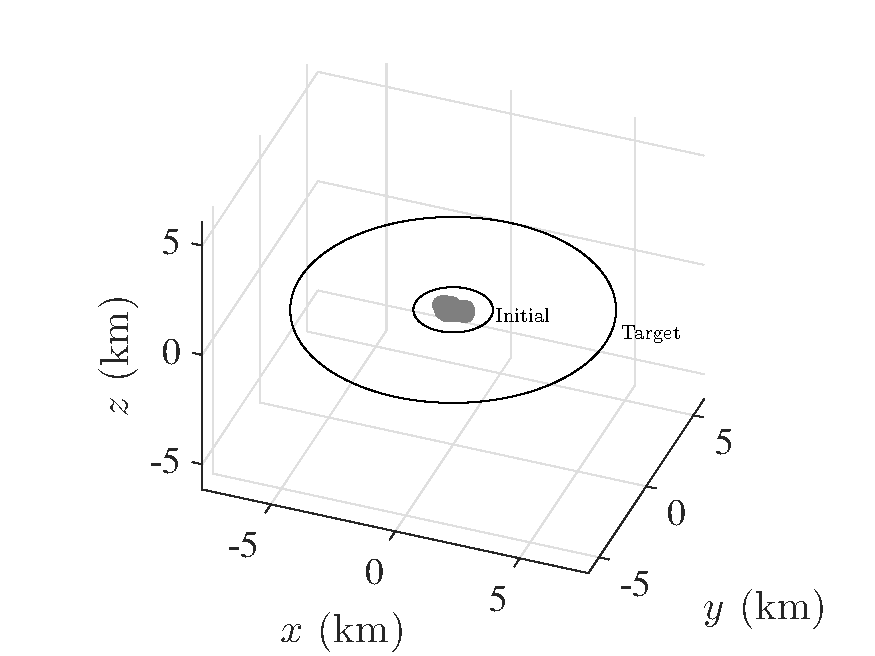
\includegraphics[width=0.5\textwidth,height=0.7\textheight,keepaspectratio]{figures/2016AAS/initial_transfer_3d.pdf}
\end{center}

\note[itemize]{
    \item Now we apply the same methodology to transfers about asteroids
}
\end{frame}%-----------------------------%

\begin{frame}{Simulation}

\begin{itemize}
    \item Generate the reachability set through discretization of \( \phi_i \)
    \item Visualize \( \Sigma \in \R^4 \) through the use of two 2-D sections
    \pause
    \item Control input allows for depature from natural dynamics
\end{itemize}

\begin{center}
    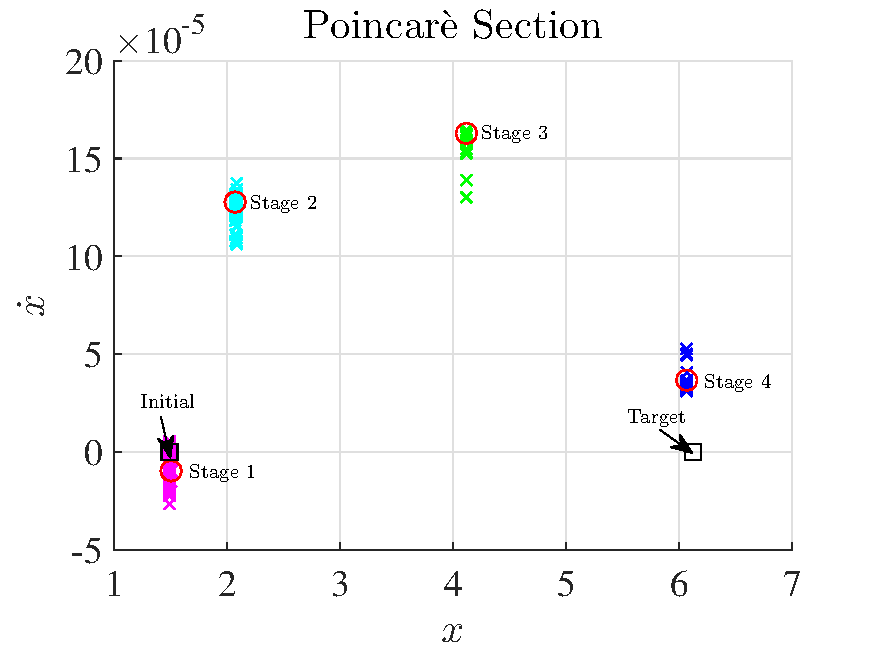
\includegraphics[width=0.5\textwidth,height=0.7\textheight,keepaspectratio]{figures/2016AAS/poincare_xvsxdot.pdf}~
    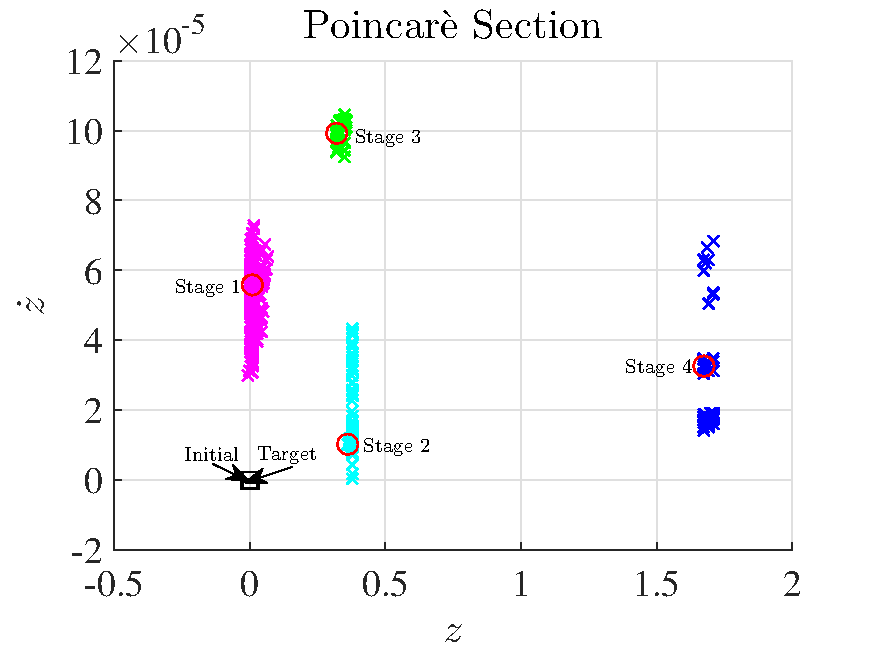
\includegraphics[width=0.5\textwidth,height=0.7\textheight,keepaspectratio]{figures/2016AAS/poincare_zvszdot.pdf}
\end{center}

\note[itemize]{
    \item This \( \Sigma \) is different than before because we're no longer dealing with a planar orbit
    \item We visualize \( \R^4\) using two two-dimensional plots
}
\end{frame}

\begin{frame}{Transfer Simulation}
    \begin{itemize}
        \item Four iterations of the reachable state to meet the target set
        \item Final transfer is computed with a fixed terminal state
    \end{itemize}

    \begin{center}
        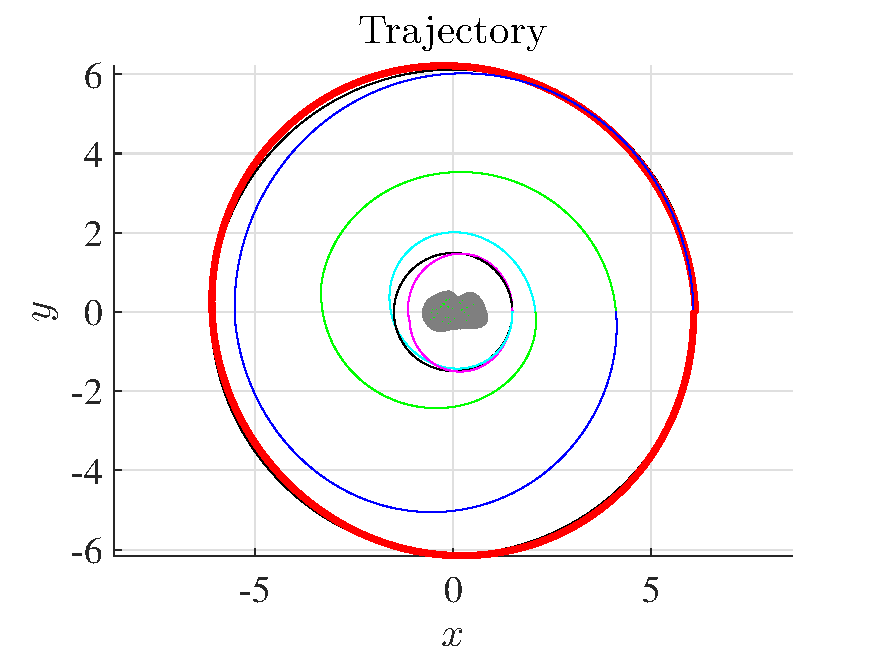
\includegraphics[width=0.5\textwidth,height=0.7\textheight,keepaspectratio]{figures/2016AAS/trajectory.pdf}~
        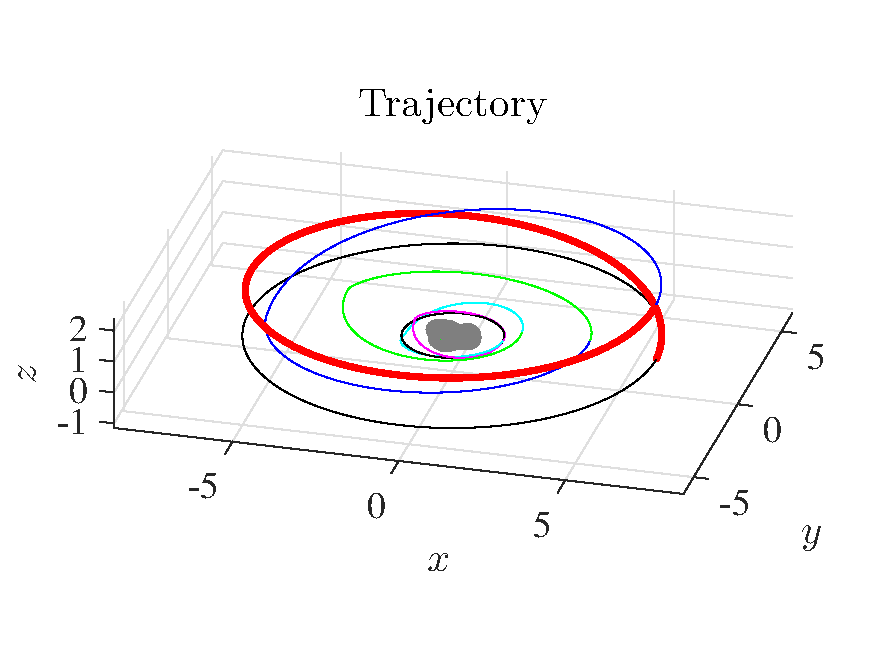
\includegraphics[width=0.5\textwidth,height=0.7\textheight,keepaspectratio]{figures/2016AAS/trajectory_3d.pdf}
    \end{center}

\end{frame}

\begin{frame}{Complete transfer}
\begin{itemize}
    \item We visualize the trajectory in body and inertial frames
\end{itemize}

\begin{center}
  \animategraphics[controls,autoplay,loop,width=0.5\textwidth,height=0.7\textheight,keepaspectratio]{60}{animation/2016AAS/body/IMG}{00500}{01499}~\hfill
  \animategraphics[controls,autoplay,loop,width=0.5\textwidth,height=0.7\textheight,keepaspectratio]{60}{animation/2016AAS/inertial/IMG}{00500}{01499}
\end{center}

\note[itemize]{
    \item we have the body frame on the left and the inertial frame on the right
}
\end{frame}
<`0`>
